\RequirePackage[OT1]{fontenc} 
\documentclass[journal]{IEEEtran}

% *** CITATION PACKAGES ***
\usepackage[style=ieee]{biblatex} 
\bibliography{example_bib.bib}    %your file created using JabRef

% *** MATH PACKAGES ***
\usepackage{amsmath}

% Table Packages
\usepackage{booktabs}
\usepackage{tabularx}

% *** PDF, URL AND HYPERLINK PACKAGES ***
\usepackage{url}
% correct bad hyphenation here
\hyphenation{op-tical net-works semi-conduc-tor}
\usepackage{graphicx}  %needed to include png, eps figures
\graphicspath{{./images/}}
\usepackage{float}  % used to fix location of images i.e.\begin{figure}[H]

\begin{document}

% paper title
\newcommand{\LabNumber}{\#10}
\newcommand{\LabTitle}{Radio Frequency Mixers}

\title{RF Lab Module \LabNumber\ --- \LabTitle}
%\\ \small{Title of the session (you can be creative highlighting your findings)}}

% author names 
\author{Stephen Campbell
    % Student 2 First Name Last Name 
}% <-this % stops a space

% The report headers
\markboth{EE/CE 4202 Electrical and Computer Engineering Laboratory in Circuits. Lab \LabNumber, \today}%do not delete next lines
{Shell \MakeLowercase{\textit{et al.}}: Bare Demo of IEEEtran.cls for IEEE Journals}

% make the title area
\maketitle

% As a general rule, do not put math, special symbols or citations
% in the abstract or keywords.
\begin{abstract}
    Overall, In this lab  overall familiarity with the key parameters and
    performance of practical RF mixer was gained. The importance of Conversion Loss
    was shown to be of tantamount significance. The non idealities of mixer's was
    evident through these precise lab measurements.
\end{abstract}

\section{Introduction}

\IEEEPARstart{T}{his} lab utilizes the spectrum analyzer, signal generator, and VNA acting as a
signal generator to determine the conversion loss of the mixer under test. The
VNA is also used to characterize the Mixer's Return Loss. An important aspect of
this lab entails accounting for the cable loss present between the signal
generator and the mixer LO. This Loss is calculated given the direct measurement
with the spectrum analyzer.

\section{Procedure}
\begin{enumerate}
    \item Characterize Mixer Return Loss
          \begin{enumerate}
              \item Setup Signal Generator as LO
                    \begin{enumerate}
                        \item f = 1GHz
                        \item AMP = 7dBm + amount adjusting for cable loss
                    \end{enumerate}
              \item Setup VNA as RF
                    \begin{enumerate}
                        \item Frequency sweep from 100kHz-4GHz
                        \item perform SOLT calibration
                    \end{enumerate}
              \item Connect Test equipment to mixer
                    \begin{enumerate}
                        \item VNA to Mixer RF
                        \item Signal Generator to Mixer LO
                        \item Connect 50 Ohm Load to mixer
                        \item Save S11 parameters
                    \end{enumerate}
          \end{enumerate}
    \item Conversion Loss Measurement
          \begin{enumerate}
              \item Setup VNA Port 1 as RF
                    \begin{enumerate}
                        \item AMP = -15dBm
                        \item F = \item3 GHz
                    \end{enumerate}
              \item Setup Signal Generator as LO
                    \begin{enumerate}
                        \item f = 1GHz
                        \item AMP = 7dBm + amount adjusting for cable loss
                    \end{enumerate}
              \item Connect Test Equipment to mixer
                    \begin{enumerate}
                        \item VNA to Mixer RF
                        \item Signal Generator to Mixer LO
                              3. Spectrum Analyzer to Mixer IF
                    \end{enumerate}
              \item Turn on Signal Generator RF POWER ON
              \item Record Significant Peaks
                    \begin{enumerate}
                        \item Record Magnitude of Peak at IF = 30MHz
                        \item Record Magnitude of Peak at RF = 1GHz
                    \end{enumerate}
              \item Repeat with Carrier frequencies of 800Mhz, 600Mhz
          \end{enumerate}
    \item Power Sweep Measurements
          \begin{enumerate}
              \item LO Power Sweep
                    \begin{enumerate}
                        \item Set RF Power to -15dBm with f=1.03GHz
                        \item Sweep LO Power w/ -2,3,7,10 dBM
                        \item Record Conversion Loss
                    \end{enumerate}
              \item RF Power Sweep
                    \begin{enumerate}
                        \item Set LO Lower to  7dBm + amount adjusting for cable loss,` GHz
                        \item Sweep RF Power w/ -15,10,-5,0
                        \item Record Conversion Loss
                    \end{enumerate}
          \end{enumerate}
\end{enumerate}

\section{Analysis}

Our cable loss throughout this lab procedure was measured to be 0.8 dBm. While
the lab procedure calls for the RF VSWR, analysis showed data collected during
the lab resulted in only the S11 only being taken at 1 single frequency. The
data displayed was taken from Jason's group and a appears to be from the Mixer's
LO Port instead of the RF Port. This is shown in Fig. \ref{fig:mixer_lo_vswr} with
the corresponding datasheet graph being shown in Fig. \ref{fig:mixer_lo_vswr_ds}. Th


\begin{figure}[hp]
    \centering
    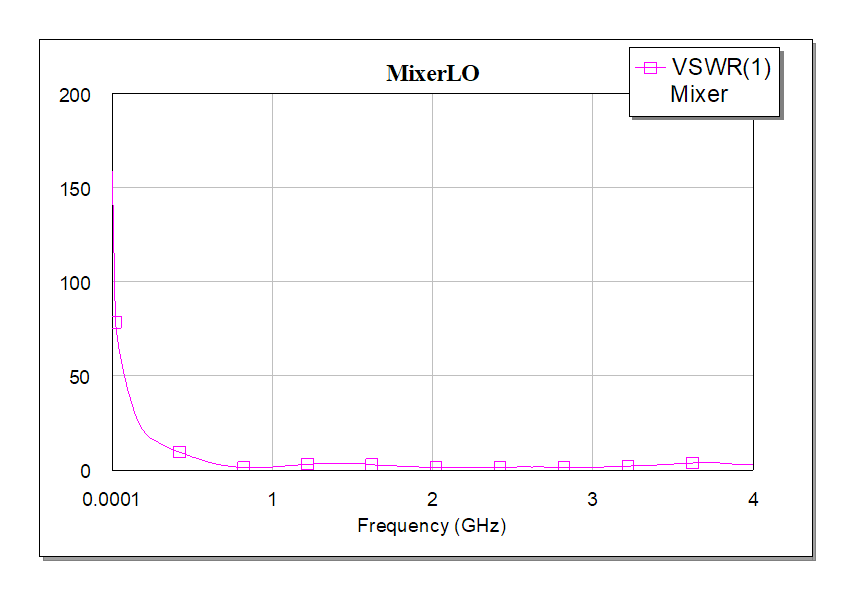
\includegraphics[width=0.3\textwidth]{mixer_lo_vswr.png}
    \caption{\label{fig:mixer_lo_vswr} Measured Mixer S11. Data taken from Jason's Group}
\end{figure}

\begin{figure}[hp]
    \centering
    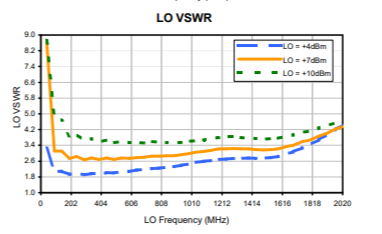
\includegraphics[width=0.3\textwidth]{mixer_lo_vswr_ds.png}
    \caption{\label{fig:mixer_lo_vswr_ds} Datasheet LO VSWR Graph }
\end{figure}

\begin{table}[]
    \centering
    \begin{tabularx}{0.5\textwidth}{XXXXXXX}
        \toprule
        Freq. (GHz) & P\_IF IF PORT & P\_RF RF PORT & Lc   & PLO IF PORT & PLO LO PORT & ISO LI \\ \midrule
        1.03        & -21.5         & -15           & -6   & -14.5       & 7           & -21.5  \\ \midrule
        0.83        & -22.2         & -15           & -7.2 & -19.25      & 7           & -26.25 \\ \midrule
        0.63        & -22.0         & -15           & -7   & -20.60      & 7           & -27.6  \\ \bottomrule
    \end{tabularx}
    \vspace{1em}
    \caption{\label{tab:conv_loss} Conversion Loss Across Frequency}

\end{table}

\begin{figure}[hp]
    \centering
    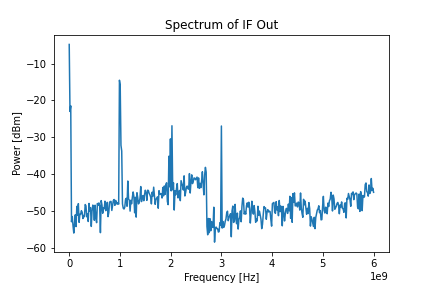
\includegraphics[width=0.3\textwidth]{spectrum_cv.png}
    \caption{\label{fig:spectrum_cv} Measured spectrum at IF port with RF at 1.03GHz}
\end{figure}

\begin{table}[hp]
    \centering
    \begin{tabular}{llll}
        \toprule
        LO power & P\_IF IF PORT & P\_RF RF PORT & Lc   \\ \midrule
        -2       & -24.6         & -15           & -9.6 \\\midrule
        3        & -22.8         & -15           & -7.8 \\\midrule
        7        & -21.6         & -15           & -6.6 \\\midrule
        10       & -21.4         & -15           & -6.4 \\ \bottomrule
    \end{tabular}
    \vspace{1em}
    \caption{f\_RF = 1.03 GHz with LO power Swept}
    \label{tab:lo_sweep}
\end{table}
\begin{table}[hp]
    \centering
    \begin{tabular}{llll}
        \toprule
        LO power & P\_IF IF PORT & P\_RF RF PORT & Lc   \\\midrule
        0        & -23.6         & -15           & -8.6 \\\midrule
        0        & -18.4         & -10           & -8.4 \\\midrule
        0        & -13.4         & -5            & -8.4 \\ \midrule
        0        & -10           & 0             & -10  \\ \bottomrule
    \end{tabular}
    \vspace{1em}
    \caption{f\_RF = 1.03 GHz with RF Power Swept}
    \label{tab:rf_sweep}
\end{table}
\begin{enumerate}

    \item  How does your measured performance of conversion loss and isolation of the mixer compare to the data sheet? (better, worse or about the same?)
          \begin{enumerate}
              \item  The Conversion Loss of the measured is 6.6dB at Lo 7dBm 1GHz, IF=30MHz. The Datasheet has the Conversion Loss at around 7.25. The Measured Result is slightly better.
              \item  The measured Isolation  is -21.5dB  at Lo 7dBm 1GHz, IF=30MHz. The datasheet is much better with -38dB Isolation at the same operating condition
          \end{enumerate}
    \item  What happens to the noise floor on the spectrum analyzer if you reduce the resolution bandwidth? How does it affect the sweep time on the spectrum analyzer?
          \begin{enumerate}
              \item  Reducing the resolution bandwidth increases the noise floor
              \item  Increasing the resolution bandwidth decreases the sweep time of the spectrum analyzer
          \end{enumerate}
    \item  Why is it important to provide the nominal LO signal power to the mixer?
          \begin{enumerate}
              \item  The LO Power directly impacts the conversion loss and signal to noise ratio of the output signal on the IF.
          \end{enumerate}
    \item  What should the signal level of the RF signal be compared to the LO signal?

          \begin{enumerate}
              \item The  RF signal should have a lower magnitude than the LO signal.
          \end{enumerate}

\end{enumerate}

The simulation was conducted using the schematic shown in Fig.
\ref{fig:sim_schem} . The output of the IF port is show in Fig.
\ref{fig:sim_spectrum}. From this graph, the Conversion Gain is -21.7 + 15 =
-6.7 dB  and the LO/IF isolation is  -20 - 7 = -27dBm.


\begin{figure}[hp]
    \centering
    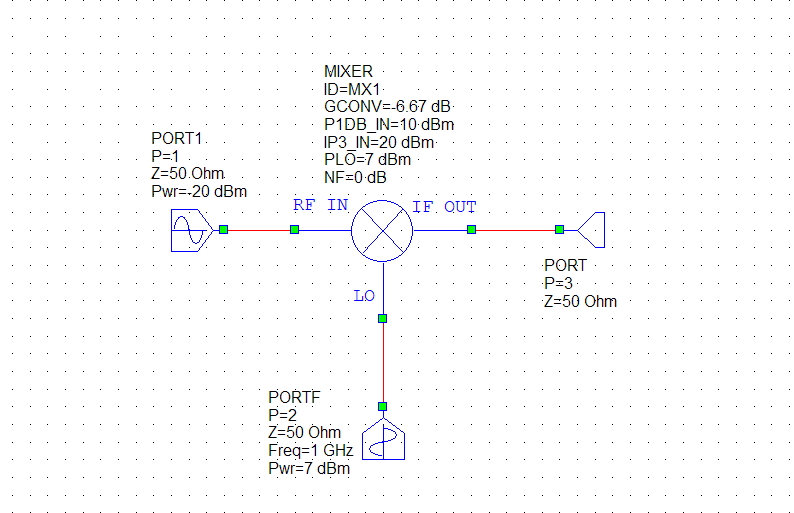
\includegraphics[width=0.3\textwidth]{sim_schem.png}
    \caption{\label{fig:sim_schem} Mixer Simulation Schematic }
\end{figure}

\begin{figure}[hp]
    \centering
    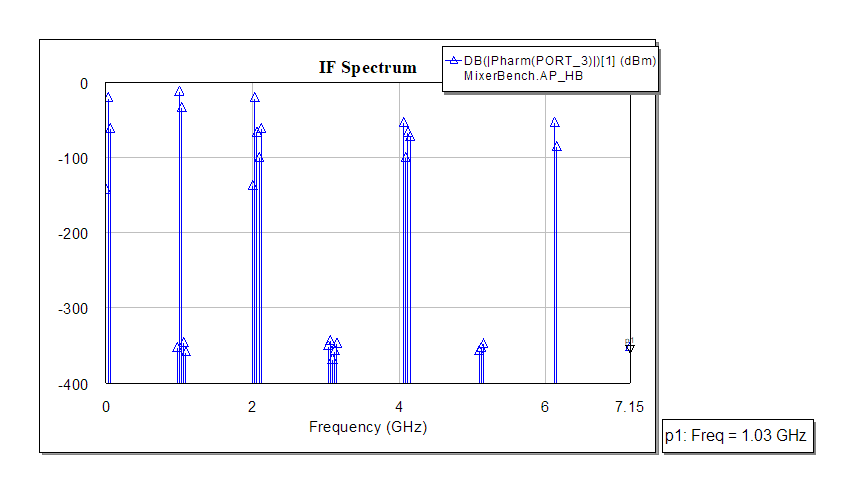
\includegraphics[width=0.3\textwidth]{sim_spectrum.png}
    \caption{\label{fig:sim_spectrum} Mixer Simulation Spectrum }
\end{figure}


\section{Discussion and Summary}

Overall, In this lab  overall familiarity with the key parameters and
performance of practical RF mixer was gained. The importance of Conversion Loss
was shown to be of tantamount significance. The non idealities of mixer's was
evident through these precise lab measurements.

\appendices
\section{Pre-Lab}
\begin{enumerate}
    \item Describe briefly what a microwave mixer is (or does).

          A mixer's main purpose is to multiply the information signal with a
          carrier bringing the information to a higher frequency. In a transmit
          case, this means moving the IF to RF w/ carrier. in the receive case
          this means bringing the RF without carrier to IF.

    \item What do the port names (RF, LO \& IF) mean? (Ex: RF=Radio Frequency)
          \begin{enumerate}
              \item RF = Radio Frequency
              \item LO = Local Oscillator
              \item IF = Intermediate Frequency
          \end{enumerate}
    \item When do we use a mixer as a down-converter in an RF system? When do we use a mixer as an up-converter?
          \begin{enumerate}
              \item a down-converter is for  receiving
              \item up-converter is for transmitting
          \end{enumerate}
    \item What is the definition (equation) for conversion loss of a down-converting RF mixer?

          \(P_{\text{out,IF}}/P_{\text{in,RF}}\)
\end{enumerate}

% \section{Extra Photos}

\end{document}